\documentclass[12pt,letterpaper]{article}

\usepackage[utf8]{inputenc}
\usepackage[spanish]{babel}
\usepackage{times}
\usepackage[left=3cm,top=2.5cm,bottom=2.5cm,right=2.5cm]{geometry}
\usepackage{graphicx}
\title{Ev\_ 1\_ 2\_ Optoacopladores\_ y\_ Relevadores}

\begin{document}

\maketitle
\


\paragraph{\large UNIVERSIDAD POLITÉCNICA DE LA ZONA METROPOLITANA DE GUADALAJARA}

\begin{figure}[h!]
\begin{center}


\includegraphics[scale=0.8]{Upzmg.png} 
\label{Upzmg}


\end{center}
\end{figure}
\

\large{Integrantes:}\\
\large{Perez de Alba Santiago Eduardo.\\
Romero Jauregui Osvaldo.\\

Fecha: 03 de Octubre del 2019.\\

Curso: Sep-Dic 2019.\\

Carrera: Ingeniería en Mecatronica.\\

Docente: Moran Garabito Carlos Enrique.\\
}

\newpage

\section{Introducción:}
\

Durante el desarrollo de esta practica se podrá observar de forma detalla el funcionamiento de cada uno de los componentes como lo son los OptoAcopladores y los relevadores, también se podrá observar el código de programación y su implementación por medio de una placa de arduino para su correcto funcionamiento.
\

\

\section{Objetivo:}
\

Representar físicamente el circuito y mostrar el paso de corriente y voltaje por medio de la placa de arduino obteniendo la activación de los relevadores y el encendido de los LEDs.
\

\section{Marco teórico:}
\
Un relevador, también conocido como relé o relay, es un interruptor cuyo control corre por cuenta de un circuito eléctrico. A través de una bobina y un electroimán incide sobre diversos contactos para la apertura o el cierre de otros circuitos, que funcionan de manera independiente. Lo que hace la bovina es crear un campo magnético que lleva los contactos a establecer una conexión. El electroimán, por su parte, permite el cierre de los contactos. De esta forma, el relevador actúa como un interruptor que puede fomentar el paso de corriente electrica o su interrupción.
\

Opto Acoplador: Es un interruptor que es activado mediante una luz infrarroja emitida por un diodo led hacia el fototransistor o cualquier otro dispositivo capaz de detectar los infrarrojos. Cuando esta luz es interrumpida o bloqueada por algún objeto el circuito se abre actuando como un interruptor abierto.
\

Arduino: Es una placa basada en un microcontrolador ATMEL. Los microcontroladores son circuitos integrados en los que se pueden grabar instrucciones, las cuales las escribes con el lenguaje de programación que puedes utilizar en el entorno Arduino IDE. Estas instrucciones permiten crear programas que interactuan con los circuitos de la placa.

\ 


\

\section{Materiales:}
\

1.-Optoacopladores 4n25\\
2.-Resistencias Varias\\
3.-Relays a 5v\\
4.-Push Buttoms\\
5.-Cables Macho-Macho(Jumpers)\\
6.-Transistor 2N2222\\
7.-Fuentes CC\\
8.-Arduino\\

\

\newpage

\section{Procedimiento:}
\

1.-Esta practica se inicio analizando el circuito otorgado con anterioridad en 2 distintos PDF y el circuito dibujado por el maestro.
\
\begin{figure}[h!]
\begin{center}
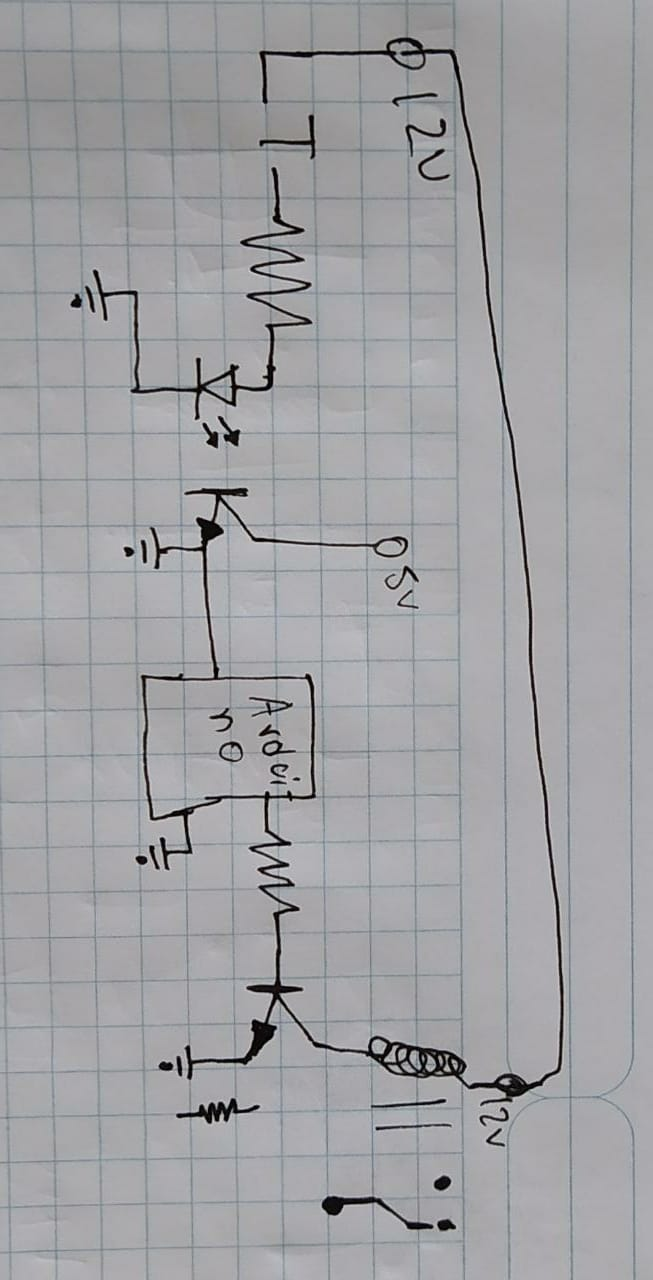
\includegraphics[width=5cm]{C1.jpeg} 
\end{center}
\end{figure}


\

2.-Lo siguiente fue iniciar el armado del circuito en físico, colocando cada uno de los componentes, basados en los archivos
\
\begin{figure}[h!]
\begin{center}
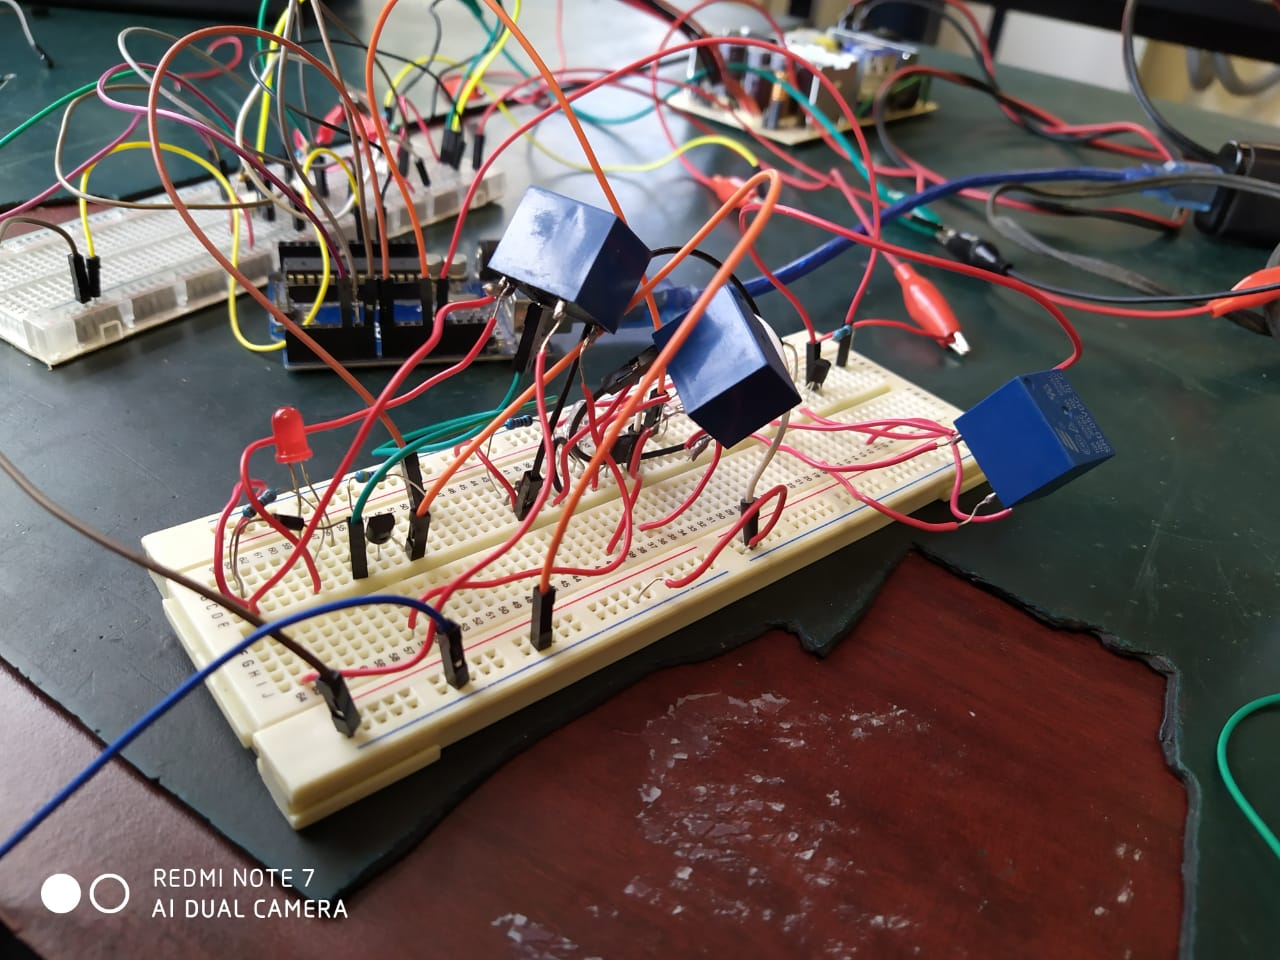
\includegraphics[width=6cm]{Circuito 1.jpeg} 
\caption{Circuito armado-Diagrama}
\end{center}
\end{figure}

\

3.-Por ultimo, se conectaron las distintas fuentes para lograr una conducción exitosa.
\


\begin{figure}[h!]
\begin{center}
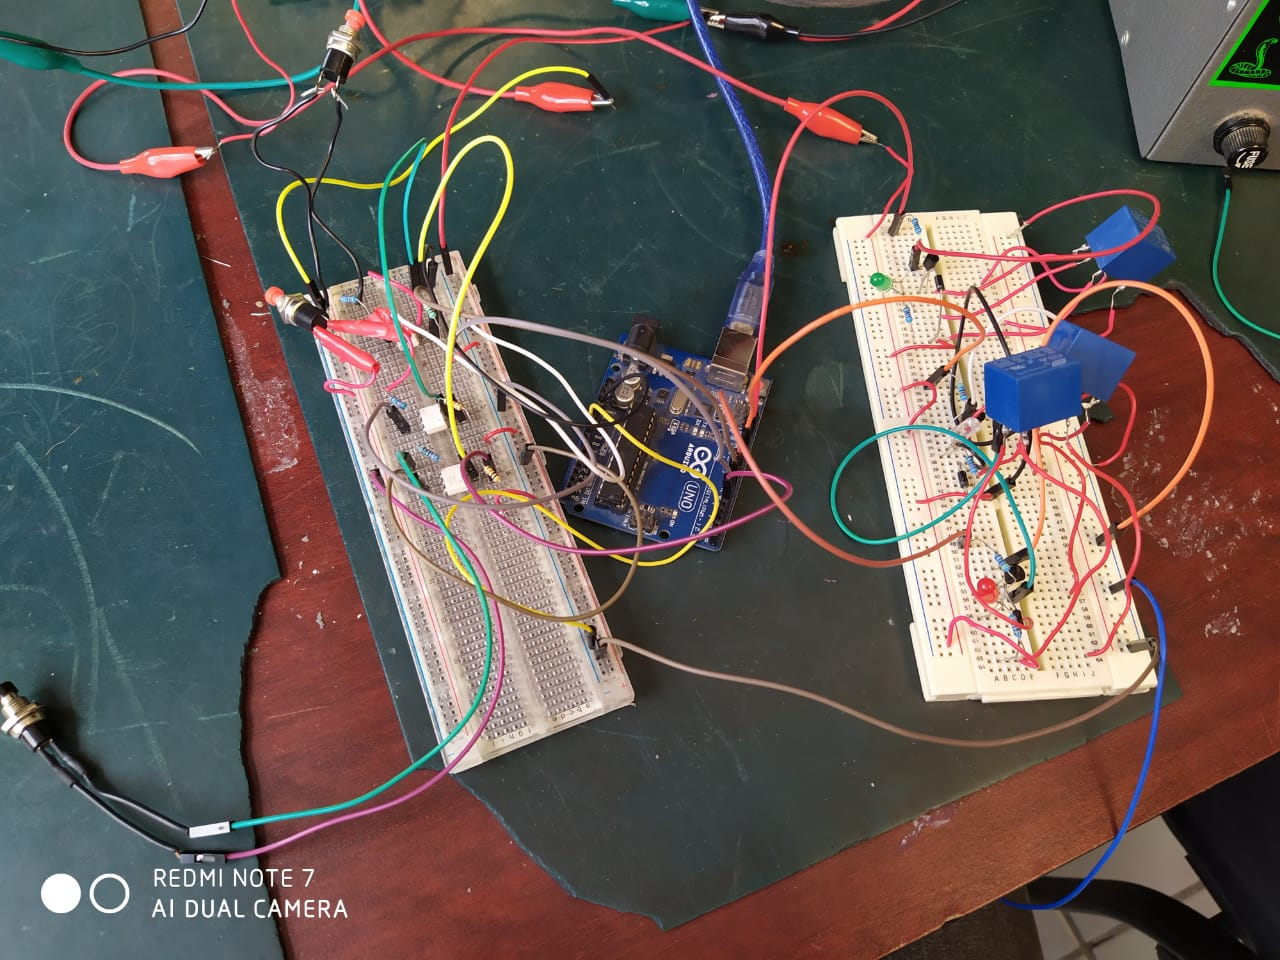
\includegraphics[width=5cm]{Circuito 2.jpeg} 
\caption{Circuito terminado}
\end{center}
\end{figure}

\

\

\section{Resultados:}
\
Como lo esperado, nuestro resultado final cae en el correcto encendido de los distintos LEDs conectados y asimismo este hace el cambio de nuestro RELAY.
\

\section{Conclusión:}
\

Durante el desarrollo de esta practica se pudo observar el funcionamiento de los optoacopladores los cuales ayudaban con la conducción y la regulación para la entrada de voltaje a la placa de arduino, como también los relevadores como función de interruptor a la salida de la placa para encender y apagar los focos LEDs y la regulación de los voltajes.







\end{document}